%% LyX 2.0.0 created this file.  For more info, see http://www.lyx.org/.
%% Do not edit unless you really know what you are doing.
\documentclass[12pt,brazil]{article}
\usepackage[T1]{fontenc}
\usepackage[utf8]{inputenc}
\usepackage{amsmath}
\usepackage{amssymb}
\usepackage{graphicx}

\makeatletter

%%%%%%%%%%%%%%%%%%%%%%%%%%%%%% LyX specific LaTeX commands.
%% A simple dot to overcome graphicx limitations
\newcommand{\lyxdot}{.}


\makeatother

\usepackage{babel}
\begin{document}

\title{Aula Exercício de Introdução ao SSH}


\author{Henrique Gemignani Passos Lima}

\maketitle
\tableofcontents{}


\section{O que é SSH, e principais características}

SSH, Secure Shell, é um protocolo de rede que permite uma conexão
segura entre dois computadores através de uma rede insegura.

Principais caracteristicas:
\begin{enumerate}
\item Autentica o servidor, impedindo ataques do estilo {}``man-in-the-middle''
\item Conexão criptografada: senhas não passam em branco pela rede
\end{enumerate}

\section{Utilidades para o SSH}


\subsection{Shell Remoto}

O principal uso do SSH é fazer um login numa máquina remota. TODO:
completar


\subsection{Transferência de Arquivos}

É possivel transmitir arquivos de uma máquina para outra por meio
do SSH através do \texttt{scp} ou \texttt{sftp.}

TODO: completar


\subsection{Túneis}

Túneis permitem encapsular protocolos inseguros na conexão segura
do SSH, como por exemplo acessar e-mails.

Também é possível utilizar túneis para burlar problemas devido ao
NAT.


\section{Como usar}

Existem diversos clientes, mas nessa aula veremos apenas dois:


\subsection{PuTTY}

Embora essa aula foque apenas na versão Windows do PuTTY, é importante
notar que esse é um programa é multi-plataforma e possui versões para
Linux. 

\begin{figure}
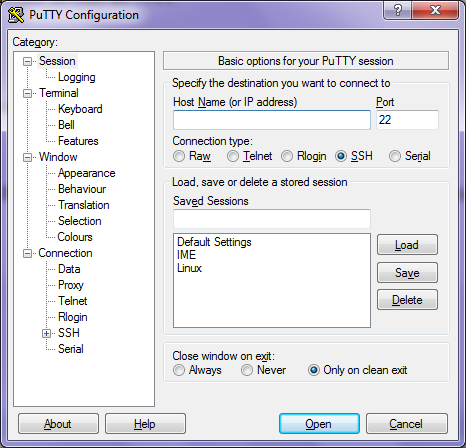
\includegraphics{putty}

\caption{Tela inicial do PuTTY}


\end{figure}





\subsection{OpenSSH Client}


\section{Métodos de Autenticação}


\subsection{Senha }

Método simples e direto ao ponto. Aparece um prompt onde você digita
a senha, que é então transmitida de maneira segura para o servidor,
que então verifica como bem quiser se a senha é válida.


\subsection{Chaves}

Uma chave SSH é composta de duas partes: a pública e a privada. Cada
parte tem um uso diferente, e juntas são utilizadas para autenticação.

Coloca-se a chave pública em todos os servidores no qual você deseja
autenticar-se, enquanto a chave privada permanece ao lado de seu cliente.

Ao especificar os parametros para abrir uma conexão SSH, você também
pode especificar o caminho para a chave privada que deseja usar. O
cliente tentará autenticar-se com o servidor usando essa chave.

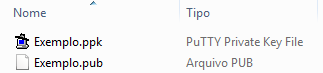
\includegraphics{privatekey}


\subsubsection{Agente SSH}


\section{Túneis }


\subsection{Local <-> Remoto }


\subsection{Remoto <-> Local }


\subsection{Dinâmico }


\subsection{X}
\end{document}
